\documentclass[tikz,border=3pt]{standalone}
\usepackage{fontspec}
\usepackage{amsmath}
\usepackage{xcolor}
\usepackage{tikz}
\usepackage{pgfplots}
\pgfplotsset{compat=1.18}
\usetikzlibrary{arrows.meta,calc,fit,positioning,shapes.geometric,shapes.misc,patterns,plotmarks}
\IfFontExistsTF{Arial}{\setsansfont{Arial}}{\setsansfont{TeX Gyre Heros}}
\renewcommand{\familydefault}{\sfdefault}
\tikzset{
  >={Stealth[length=2.2mm,width=1.5mm]},
  exact title/.style={font=\bfseries\fontsize{10.5}{12}\selectfont,align=center},
  exact subtitle/.style={font=\fontsize{6.3}{7.2}\selectfont,align=center},
  exact label/.style={font=\fontsize{6.4}{7.5}\selectfont,align=center},
  exact tiny/.style={font=\fontsize{5.3}{6.3}\selectfont,align=center},
  panel/.style={draw=black!14,rounded corners=1.2mm,fill=white,line width=.45pt},
  neutral/.style={draw=black!30,fill=black!3,rounded corners=1mm,line width=.45pt},
  arrow/.style={-Stealth,line width=.7pt},
  softarrow/.style={-Stealth,line width=.55pt,draw=black!45},
  dashedarrow/.style={-Stealth,dashed,line width=.55pt,draw=black!55},
  metric/.style={font=\fontsize{5.3}{6.3}\selectfont,fill=white,inner sep=1pt},
}
\newcommand{\pill}[4]{\node[draw=#2!70,fill=#2!10,rounded corners=1.5mm,inner xsep=3pt,inner ysep=2pt,exact label,text=#2] (#1) at #3 {#4};}
\newcommand{\frameboxx}[4]{\draw[draw=#2!65,fill=#2!8,rounded corners=.6mm,line width=.5pt] (#1.south west) rectangle (#1.north east);\node[exact tiny,text=#2] at #3 {#4};}
\newcommand{\axislabel}[3]{\node[exact tiny,text=black!60] at (#1) {#2};\node[exact tiny,text=black!60,rotate=90] at (#3) {#2};}

\definecolor{mosgray}{HTML}{8B949E}\definecolor{mosteal}{HTML}{2A9D8F}\definecolor{mosviolet}{HTML}{7B61A8}\definecolor{mosamber}{HTML}{E9C46A}\definecolor{mosink}{HTML}{263238}
\begin{document}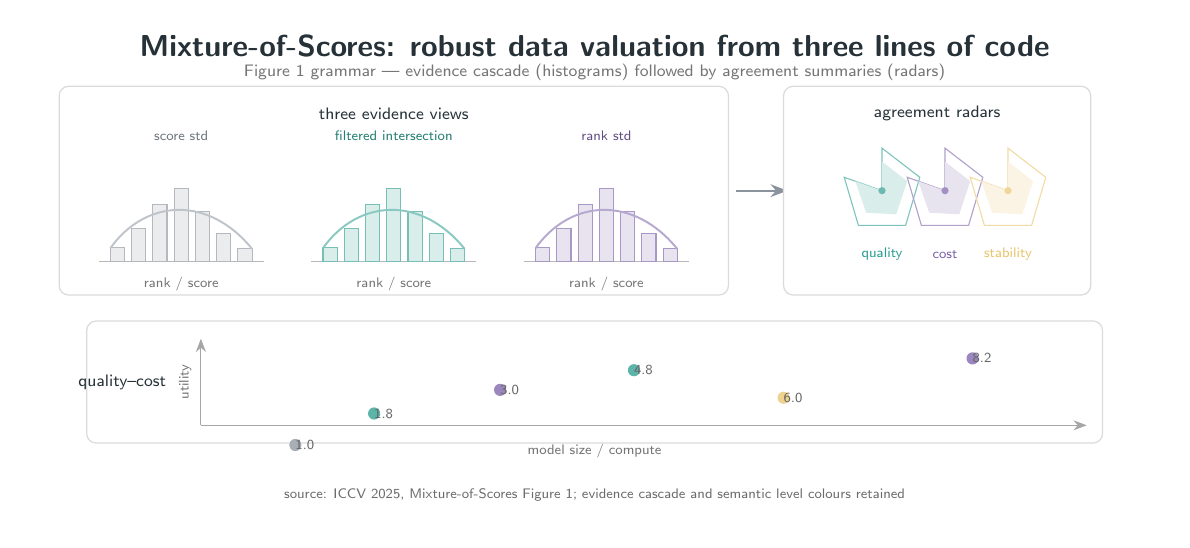
\begin{tikzpicture}[x=1cm,y=1cm]
\path[use as bounding box] (-.2,-4.0) rectangle (14.2,2.25);
\node[exact title,text=mosink] at (7,2.02) {Mixture-of-Scores: robust data valuation from three lines of code};
\node[exact subtitle,text=black!54] at (7,1.68) {Figure 1 grammar — evidence cascade (histograms) followed by agreement summaries (radars)};
\node[panel,minimum width=8.5cm,minimum height=2.65cm] at (4.45,.18) {};
\node[exact label,text=mosink] at (4.45,1.16) {three evidence views};
\foreach \x/\title/\c in {1.75/score std/mosgray,4.45/filtered intersection/mosteal,7.15/rank std/mosviolet}{\node[exact tiny,text=\c!80!black] at (\x,.88) {\title};\draw[black!28] (\x-1.05,-.72) -- (\x+1.05,-.72);\foreach \i/\hh in {0/.18,1/.42,2/.72,3/.93,4/.64,5/.36,6/.16}{\draw[\c!65,fill=\c!18] (\x-.9+\i*.27,-.72) rectangle (\x-.72+\i*.27,-.72+\hh);}\draw[\c!55,line width=.7pt] (\x-.9,-.55) .. controls (\x-.45,.08) and (\x+.35,.12) .. (\x+.9,-.56);\node[exact tiny,text=black!54] at (\x,-1.0) {rank / score};}
\draw[arrow,draw=mosgray] (8.8,.18) -- (9.45,.18);\node[panel,minimum width=3.9cm,minimum height=2.65cm] at (11.35,.18) {};
\node[exact label,text=mosink] at (11.35,1.16) {agreement radars};
\foreach \cx/\cy/\c in {10.65/.18/mosteal,11.45/.18/mosviolet,12.25/.18/mosamber}{\draw[\c!60] (\cx,\cy) -- +(0,.54) -- +(0.48,.17) -- +(0.3,-.44) -- +(-.3,-.44) -- +(-.48,.17) -- cycle;\fill[\c!18] (\cx,\cy) -- +(0,.37) -- +(0.32,.12) -- +(0.18,-.3) -- +(-.2,-.28) -- +(-.34,.12) -- cycle;\fill[\c!70] (\cx,\cy) circle (1.3pt);}\node[exact tiny,text=mosteal] at (10.65,-.63) {quality};\node[exact tiny,text=mosviolet] at (11.45,-.63) {cost};\node[exact tiny,text=mosamber] at (12.25,-.63) {stability};
\node[panel,minimum width=12.9cm,minimum height=1.55cm] at (7,-2.25) {};
\node[exact label,text=mosink] at (1.0,-2.25) {quality–cost};\draw[black!35,-Stealth] (2.0,-2.8) -- (13.25,-2.8);\draw[black!35,-Stealth] (2.0,-2.8) -- (2.0,-1.7);\foreach \x/\y/\s/\c in {3.2/-.25/1.0/mosgray,4.2/.15/1.8/mosteal,5.8/.45/3.0/mosviolet,7.5/.7/4.8/mosteal,9.4/.35/6.0/mosamber,11.8/.85/8.2/mosviolet}{\fill[\c!76] (\x,\y-2.8) circle (2.2pt);\node[exact tiny,text=black!60] at (\x+.12,\y-2.8) {\s};}\node[exact tiny,text=black!55] at (7,-3.13) {model size / compute};\node[exact tiny,text=black!55,rotate=90] at (1.8,-2.25) {utility};
\node[exact tiny,text=black!58] at (7,-3.68) {source: ICCV 2025, Mixture-of-Scores Figure 1; evidence cascade and semantic level colours retained};
\end{tikzpicture}\end{document}
